\documentclass[conference]{IEEEtran}
\IEEEoverridecommandlockouts
\usepackage{cite}
\usepackage{amsmath,amssymb,amsfonts}
\usepackage{algorithmic}
\usepackage[ruled]{algorithm2e}
\usepackage{graphicx}
\usepackage{textcomp}
\usepackage{xcolor}
\usepackage{float}
\usepackage[colorlinks, urlcolor=blue]{hyperref}
\graphicspath{{./Pictures/}}
\def\BibTeX{{\rm B\kern-.05em{\sc i\kern-.025em b}\kern-.08em
    T\kern-.1667em\lower.7ex\hbox{E}\kern-.125emX}}
\begin{document}


\title{Perkalian Matriks dengan Beberapa Algoritma}

\author{\IEEEauthorblockN{Surya Dharma*, Fariz Iftikhar Falakh†, Senggani Fatah Sedayu§}
\IEEEauthorblockA{\textit{School of Electrical Engineering and Informatics} \\
\textit{Institut Teknologi Bandung}\\
Bandung, Indonesia\\
\{*13220027, †13220029, §13220035\}@std.stei.itb.ac.id}
}

\maketitle

\begin{abstract}
Metode perkalian matriks yang umumnya diketahui adalah dengan perkalian baris kolom (dalam pemrograman perkalian baris kolom disebut \textit{Naive algorithm}).
Dengan berkembangnya ilmu matematika dan komputasi, diperoleh beberapa algoritma perkalian matriks yang memakan lebih sedikit waktu dibandingkan \textit{Naive algorithm}).
Penulis akan menggunakan beberapa algoritma untuk menghitung hasil perkalian 2 buah matriks dengan ukuran besar.
Lalu penulis akan membandingkan kompleksitas waktu dari algoritma-algoritma tersebut dengan menganalisis kompleksitas waktu dan ruang.
\end{abstract}

\begin{IEEEkeywords}
matriks, \textit{Naive algorithm}, algoritma Strassen, algoritma Cannon
\end{IEEEkeywords}

\section{Pendahuluan}
Perkalian matriks merupakan suatu operasi biner dengan operan dua buah matriks yang menghasilkan sebuah matriks.
Perkalian matriks memiliki peran penting dalam dunia matematika serta memiliki jangkauan aplikasi yang sangat luas, misalnya \textit{signal processing}).
Karena banyaknya kegunaan operasi ini, matematikawan mencoba untuk mencari metode perkalian matriks yang lebih memakan sedikit waktu.
Dari usaha tersebut, banyak metode yang dikembangkan agar perkalian matriks---terutama untuk matriks dengan ukuran besar---menjadi lebih efisien.

Algoritma-algoritma yang digunakan oleh penulis adalah \textit{Naive algorithm}, algoritma Strassen, dan algoritma Cannon.
Ketiga algoritma tersebut akan diimplementasikan dalam bahasa pemrograman C.
Penulis akan membandingkan seberapa cepat suatu algoritma menyelesaikan hasil perkalian 2 buah matriks dengan algoritma lain.

\section{Studi Pustaka}
\subsection{Naive Algorithm}
Naive algorithm seperti namanya, merupakan sebuah algoritma yang sangat polos di mana pada algoritma ini kita akan mengkalkulasikan setiap \textit{entry} menjadi sebuah \textit{sum of product}. Karena hal inilah \textit{Naive Algorithm} memiliki lebih banyak perhitungan dibandingkan algoritma-algoritma perkalian matriks lainnya. Pada algoritma, untuk sebuah matriks $n\times n$ yang dikalikan dengan matriks berukuran $n\times n$ lainnya, algoritma ini membutuhkan $n^3$ perhitungan, sehingga time complexity dari algoritma ini adalah \textit{O($n^3$)}.

\subsubsection{Source Code Naive Algorithm}
\begin{algorithm}
    \caption{Naive Algorithm}
    \KwIn{Matriks A, matriks B ukuran $n \times n$}
    \KwOut{Matriks C ukuran $n \times n$}
    \KwSty{Procedure}\\
    \For{$i = 0$ \KwTo $n$}{
        \For{$j = 0$ to \KwTo $n$}{
            $C[i][j] = 0$\\
            \For{$k = 0$ \KwTo $n$}{
                $C[i][j] = C[i][j] + A[i][k] \cdot B[k][j]$
            }
        }
    }
\end{algorithm}

\subsection{Strassen Algorithm}
Algoritma Strassen merupakan algoritma untuk mencari hasil perkalian yang lebih cepat dibanding dengan Algoritma naive.
Algoritma Naive melakukan perhitungan perkalian matriks biasa yang memerlukan $n^3$ perhitungan, sedangkan untuk Algoritma Strassen memerlukan $n^(2.81)$ perhitungan. 
Berkurangnya banyak perhitungan disebabkan oleh penggunaan pengurangan dan penjumlahan pada perhitungan sebelumnya untuk mendapat nilai baru.
Karena proses pengurangan dan penjumlahan lebih ringan dibanding dengan perkalian, maka time complexity dari algoritma menurun.

\subsubsection{Source Code Strassen Algorithm}
\begin{algorithm}
    \caption{KaliStrassen(A, B : matriks, n : \textbf{integer})}
	\KwIn{Matriks A, matriks B, dan ukuran matriks}
	\KwOut{Hasil perkalian A dan B}
    \KwSty{Algorithm}\\
	\eIf{n = 1}{
        \textbf{return} A $\ast$ B
    }{
        Bagi A menjadi A11, A12, A21, dan A22 dengan ukuran $n/2 \times n/2$\\
        Bagi B menjadi B11, B12, B21, dan B22 dengan ukuran $n/2 \times n/2$\\
        M1 $\leftarrow$ KaliStrassen(A12 - A22, B21 + B22, $n/2$)\\
        M2 $\leftarrow$ KaliStrassen(A11 + A22, B11 + B22, $n/2$)\\
        M3 $\leftarrow$ KaliStrassen(A11 - A21, B11 + B12, $n/2$)\\
        M4 $\leftarrow$ KaliStrassen(A11 + A12, B22, $n/2$)\\
        M5 $\leftarrow$ KaliStrassen(A11, B12 - B22, $n/2$)\\
        M6 $\leftarrow$ KaliStrassen(A22, B21 - B11, $n/2$)\\
        M7 $\leftarrow$ KaliStrassen(A21 + A22, B11, $n/2$)\\
        C11 $\leftarrow$ M1 + M2- M4 + M6\\
        C12 $\leftarrow$ M4 + M5\\
        C21 $\leftarrow$ M6 + M7\\
        C22 $\leftarrow$ M2 - M3 + M5 - M7\\
        \textbf{return} C \{C gabungan C11, C12, C21, dan C22\}
    }
\end{algorithm}

\subsection{Cannon Algorithm}
Dalam \textit{computer science}, algoritma Cannon adalah algoritma terdistribusi (dirancang untuk dilakukan pada \textit{hardware} komputer yang terdiri dari berbagai prosesor)
untuk perkalian matriks untuk mesh (jaringan yang terbentuk dari sel dan titik) 2 dimensi.
Algoritma ini cocok digunakan untuk mesh N*N (atau matriks N*N) dan tidak cocok digunakan untuk matriks bukan persegi.
Modifikasi matriks dengan algoritma Cannon berhubungan dengan geser sirkular (\textit{circular shift}).
Geser sirkular adalah operasi menggeser elemen-elemen array (atau matriks), mirip seperti \textit{bit shifting}.
Misalnya digunakan kasus geser sirkular kiri dan \textit{bit shiifting} ke kiri.
Perbedaannya adalah dengan \textit{bit shiifting}, elemen paling kiri akan hilang, 
sementara dengan geser sirkular kiri, elemen paling kiri akan dipindahkan ke paling kanan.

\subsubsection{Source Code Cannon Algorithm}
\begin{algorithm}
    \caption{Algoritma Cannon}
    \KwResult{Hasil perkalian matriks A berukuran n*n dan matriks B berukuran n*n}
    \KwSty{Procedure}\\
    \For{$i = 0$ \KwTo $n - 1$}{
        Geser sirkular kiri $baris[i]$ A $i$ kali
    }
    \For{$i = 0$ \KwTo $n - 1$}{
        Geser sirkular atas $kolom[i]$ B $i$ kali
    }
    \For{$k = 0$ \KwTo $n - 1$}{
        \For{$i = 0$ \KwTo $n - 1$}{
            \For{$j = 0$ \KwTo $n - 1$}{
                $C[i][j] \leftarrow C[i][j] + A[i][j] \times B[i][j]$
            }
        }
        Geser sirkular kiri semua baris A 1 kali\\
        Geser sirkular atas semua baris B 1 kali
    }
\end{algorithm}

\begin{figure}[h]
    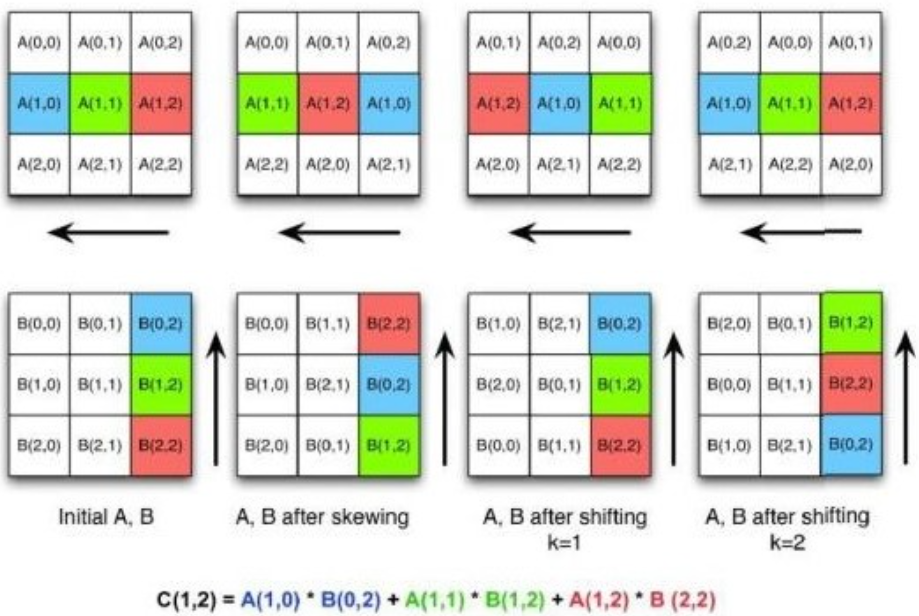
\includegraphics[width = 8cm, height = 6cm]{Ilustrasi_algoritma_cannon.png}
    \centering
    \caption{Ilustrasi algoritma Cannon}
\end{figure}

\subsection{Kompleksitas}
Ada banyak hal yang harus dipertimbangkan dalam membuat sebuah program.
Salah satunya adalah cara/algoritma implementasinya yang bergantung pada ukuran input.
Untuk membandingkan performa beberapa algoritma, digunakan analisis asimtotik.
Ada 3 jenis notasi untuk menyatakan kompleksitas algoritma, yaitu notasi $\Theta$ (theta), notasi \textit{Big O}, dan notasi $\Omega$ (omega).

Notasi \textit{Big O} menyatakan batas atas asimtotik dari kompleksitas suatu algoritma.
Notasi $\Omega$ menyatakan batas bawah asimtotik dari kompleksitas suatu algoritma.
Notasi $\Theta$ merupakan gabungan notasi \textit{Big O} dan Notasi $\Omega$.
Notasi yang biasanya digunakan adalah notasi \textit{Big O}.

Definisi \textit{Big O} secara formal adalah ada suatu fungsi $T$ yang memenuhi
$T(n) = O(f(n))$ jika terdapat suatu konstanta $c$ dan $N_0$ sehingga $T(n) \le c \cdot f(n)$ untuk semua $n \ge N_0$.
Dalam penulisan notasi, pengguna hanya fokus pada bagian dominan dari sebuah fungsi kompleksitas.
Misal terdapat sebuah fungsi $T(n) = n^2 + n + 1$.
Karena $n^2$ tumbuh lebih cepat dibandingkan dengan $n$ dan 1 untuk input n yang makin besar, 
maka notasi \textit{Big O} dari $T(n)$ adalah $O(n^2)$.
Cara lain untuk menentukan \textit{Big O} dari $T(n)$ adalah dengan menggunakan definisi notasi \textit{Big O}.
Pilih $f(n) = N^2$, $c = 2$, dan $N_0 = 2$, maka $T(n)$ akan selalu lebih kecil dari $c \cdot f(n)$ untuk semua $n \ge N_0$ 
sehingga diperoleh notasi \textit{Big O} dari $T(n)$ yaitu $O(n^2)$.

\begin{figure}[h]
   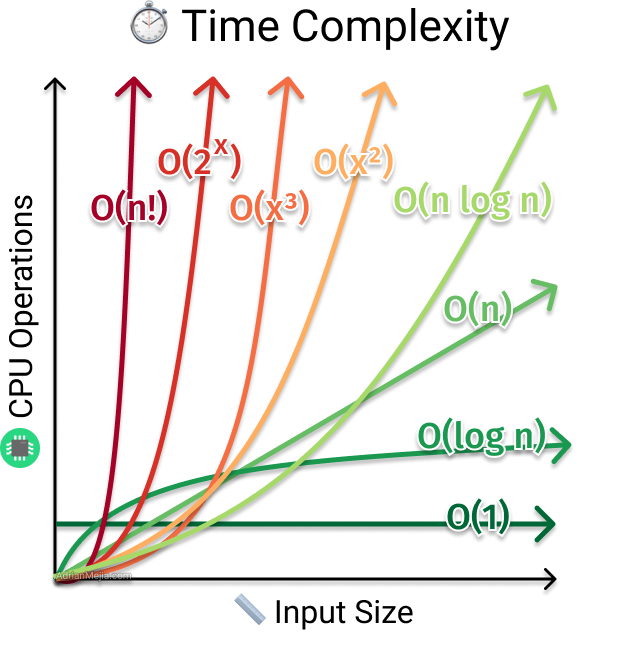
\includegraphics[width = 6cm, height = 5cm]{Kurva_Kompleksitas_Waktu.png}
   \centering
   \caption{Kurva perbandingan kompleksitas waktu suatu algoritma}
\end{figure}

\section{Metodologi Penelitian}
ini metodologi

\section{Implementasi dan Pengujian}

\subsection{Implementasi Naive Algorithm pada Bahasa C}
Untuk mengimplementasikan \textit{Naive algorithm} pada C, diperlukan beberapa prosedur, yaitu : Deklarasi Matriks, pengisian nilai matriks, pencetakan matriks sebelum dikalikan, perkalian matriks, serta pencetakan matriks hasil perkalian. 

\subsubsection{Deklarasi Matriks}
Deklarasi matriks merupakan sebuah prosedur di mana user bisa memilih ukuran dari matriks yang ingin dikalikan. Lalu karena ukurannya yang belum pasti serta range ukuran matriks yang bisa menjadi sangat besar, maka digunakan \textit{dynamic memory}.
\subsubsection{Pengisian nilai matriks}
Prosedur ini akan mengisi nilai matriks yang sebelumnya telah kita deklarasikan ukurannya dengan menggunakan fungsi random, di mana program akan mengisi setiap \textit{cell} pada matriks dengan nilai random yang berkisar di range 0-9.
\subsubsection{Cetak Matriks Sebelum Dikalikan}
Prosedur ini fungsinya sebenarnya hanya untuk pengecekan manual perkalian matriks. Prosedur ini akan mencetak nilai-nilai dari kedua matriks yang sebelumnya telah diisi secara random oleh program.
\subsubsection{Perkalian Matriks}
Prosedur ini akan mencari nilai dari perkalian dua matriks yang memiliki ukuran yang sama ($n\times n$) dengan menggunakan metode \textit{Naive algorithm}.
\subsubsection{Cetak Matriks Hasil Perkalian}
Prosedur ini akan mencetak hasil perkalian dua matriks yang sebelumnya telah dikalikan pada prosedur perkalian matriks.

\subsection{Implementasi Strassen Algorithm pada Bahasa C}

\subsection{Implementasi Cannon Algorithm pada Bahasa C}
Ada 7 prosedur yang digunakan untuk mengimplementasikan algoritma Cannon, 1 untuk inisialisasi matriks, 1 untuk mencetak isi matriks (untuk keperluan \textit{debugging}), 
4 untuk memodifikasi elemen matriks, dan 1 untuk mengisi matriks hasil.
Inisialisasi matriks pada dasarnya mengisi 2 matriks dengan nilai dalam rentang 0 - 9.
Pengisian matriks hasil diimplementasikan dengan \textit{nested loop} indeks baris dan kolom, 
lalu elemen matriks C baris ke-$i$ kolom ke-$j$ didapatkan dari perkalian elemen matriks A baris ke-$i$ kolom ke-$j$ dan elemen matriks B baris ke-$i$ kolom ke-$j$.

Prosedur yang digunakan untuk memodifikasi elemen matriks adalah geser sirkular kiri baris, geser sirkular atas kolom, geser sirkular kiri matriks, dan geser sirkular atas matriks.
Geser sirkular kiri baris diimplementasikan dengan menyimpan elemen pertama array (misalnya di variabel $temp$), lalu dilakukan \textit{looping} untuk menukar elemen array.
Setelah itu, elemen array paling terakhir akan disubstitusikan dengan nilai dari $temp$.
Geser sirkular atas kolom diimplementasikan dengan cara yang mirip, hanya berbeda pada parameter fungsi dan pengaksesan array saja.
Geser sirkular kiri matriks diimplementasikan dengan menyimpan elemen kolom 0 (misalnya di array $arr\_temp$), lalu dilakukan \textit{looping} untuk menukar elemen setiap baris.
Setelah itu, kolom terakhir matriks akan diisi oleh array $arr\_temp$ sesuai indeksnya.
Geser sirkular atas matriks diimplementasikan dengan cara yang mirip, 
perbedaannya adalah geser sirkular kiri menyimpan elemen kolom 0, sedangkan geser sirkular atas menyimpan elemen baris 0.
Implementasi algoritma ini dalam bahasa pemrograman C dapat dilihat di
\href{https://github.com/Fariz06/Tugas-5-PMC}{sini}.

\section{Kesimpulan}
Kesimpulannya pusing tujuh keliling

\begin{thebibliography}{00}
\bibitem{b1} G. Eason, B. Noble, and I. N. Sneddon, ``On certain integrals of Lipschitz-Hankel type involving products of Bessel functions,'' Phil. Trans. Roy. Soc. London, vol. A247, pp. 529--551, April 1955.
\bibitem{b2} J. Clerk Maxwell, A Treatise on Electricity and Magnetism, 3rd ed., vol. 2. Oxford: Clarendon, 1892, pp.68--73.
\bibitem{b3} I. S. Jacobs and C. P. Bean, ``Fine particles, thin films and exchange anisotropy,'' in Magnetism, vol. III, G. T. Rado and H. Suhl, Eds. New York: Academic, 1963, pp. 271--350.
\bibitem{b4} K. Elissa, ``Title of paper if known,'' unpublished.
\bibitem{b5} R. Nicole, ``Title of paper with only first word capitalized,'' J. Name Stand. Abbrev., in press.
\bibitem{b6} Y. Yorozu, M. Hirano, K. Oka, and Y. Tagawa, ``Electron spectroscopy studies on magneto-optical media and plastic substrate interface,'' IEEE Transl. J. Magn. Japan, vol. 2, pp. 740--741, August 1987 [Digests 9th Annual Conf. Magnetics Japan, p. 301, 1982].
\bibitem{b7} M. Young, The Technical Writer's Handbook. Mill Valley, CA: University Science, 1989.
\end{thebibliography}

\end{document}
